\newpage
\chapter{MARCO TEÓRICO CONCEPTUAL}
\section{Antecedentes}
\subsection{Antecedentes internacionales}

\cite{haquehua2025modelo} desarrollaró el trabajo \textsl{''Modelo de inventarios aplicado al control de almacén del centro de salud integral La Fuente del Cusco, 2024''} en donde esta plantilla fue realizada. Si deseas ver el trabajo de investigación subido, ingresa al siguiente link \url{https://repositorio.unsaac.edu.pe/handle/20.500.12918/11440}

\subsection{Antecedentes nacionales}
Asimismo el trabajo de investigación puede utilizar la citación entre paréntesis de la siguiente forma \citep{haquehua2025modelo}

\subsection{Antecedentes locales}

\lipsum[1]

\lipsum[1][1-3]

\section{Bases Teóricas}

Asimismo en la plantilla se pueden incluir figuras, tablas y fórmulas, una recomendación es conocer el entorno para integrar figuras y tablas. Los ejemplos se muestran a continuación:

Como se muestra en la Figura \ref{fig:img1}.
\begin{figure}[H]
  \caption{Conducta de inventario en el modelo clásico económica de pedido (EOQ)}
  {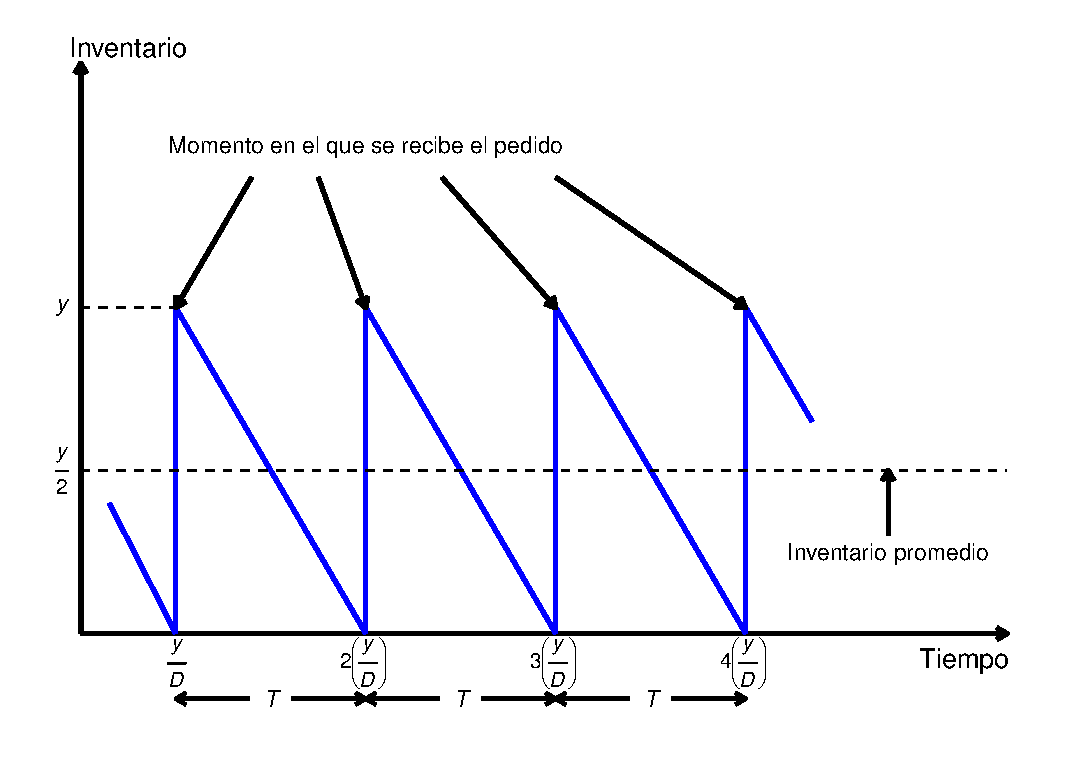
\includegraphics[width=13.5cm, height=8cm]{images/img1.pdf}}
  \caption*{\textbf{Fuente:} \citep{haquehua2025modelo}}
  \label{fig:img1}
\end{figure}

Asimismo para colocar una tabla se usa el siguiente comando, la Tabla \ref{table:ABC_resumen} resume el análisis ABC.
\begin{table}[h!]
    \caption{Resumen de actividades basadas en costos (ABC)}
    \begin{tabular}{p{0.8cm} p{2.52cm} p{5.2cm} p{4.9cm}}
        \hline
        \textbf{Grupo} & \textbf{$(\%)$ de Costos} & \textbf{$(\%)$ ocupación del inventario} & \textbf{Usar técnicas cuantitativas} \\
        \hline
        \textbf{A} & $70\%$ & $10\%$ & Si \\
        \textbf{B} & $20\%$ & $20\%$ & Los que tienen costos altos \\
        \textbf{C} & $10\%$ & $70\%$ & No \\
        \hline
    \end{tabular}
    \label{table:ABC_resumen}
\end{table}

Para insertar definiciones, teoremas y corolarios usamos el siguiente esquema

\begin{definition}
	Sea $\mathbf{f}: D \rightarrow \mathbb{R}^m$, donde $D \subset \mathbb{R}^n$, entonces se dice que $\mathbf{f(x)}$ tiene un límite $\mathbf{L}=({L}_{1},{L}_{2}, \cdots , {L}_{m})$ donde $\mathbf{x}$ se aproxima hacia $\mathbf{a}$, descrito como $\mathbf{x} \rightarrow \mathbf{a}$, donde $\mathbf{a}$ es un punto límite de $D$, si para cada $\epsilon > 0$ existe un $\delta > 0$ tal que $\| \mathbf{f(x) - L} \| < \epsilon$ para todos los $\mathbf{x}$ en $D \cap {N}_{\delta}^{d}(\mathbf{a})$ donde ${N}_{\delta}^{d}(\mathbf{a})$ es una vecindad de $\mathbf{a}$ de radio $\delta$. Descrito de la forma $\lim_{\mathbf{x} \to \mathbf{a}} \mathbf{f(x) = L}$
\end{definition}

\begin{theorem}
	Sea $f$ definida en un punto $x_0$. Si $f$ tiene una derivada en $x_0$, entonces es continuo en $x_0$
\end{theorem}

\begin{corolary}
    Sea esto un corolario en $f$
\end{corolary}

Insertar ecuaciones

\begin{equation}
    A = B + C
\end{equation}

\section{Marco conceptual}
\noindent
\textbf{Primer marco:} \lipsum[1][1-2] \citep{haquehua2025modelo}\vspace{0.25cm}

\noindent
\textbf{Segundo marco:} \lipsum[1][1-2] \citep{haquehua2025modelo}\vspace{0.25cm}






















